\thispagestyle{myheadings}
\chapter{帰宅同行支援システム「leaving-match」}
本章では提案する帰宅同行支援システム「leaving-match」について述べる．
本システムは，ユーザ間の帰宅時刻を近づけるきっかけを提供する設計であり，この意図を反映して「退出（leaving）」と「一致（match）」を組み合わせ命名した．
以上を踏まえ，帰宅同行を促すために設計したシステムの構成と，その内部で用いられる帰宅推奨時刻の算出処理，およびユーザに対する提示・投票の仕組みについて述べる．
本研究では時刻算出手法そのものではなく，算出結果を用いたコミュニケーション支援に重点を置く．

% \section{提案システムの設計方針}
\section{提案システムの要件}
本システムは，帰宅時の偶発的な対面コミュニケーションの促進を目的とし，その実現にあたりユーザの自由意思の尊重，心理的負担の低減，および個人のプライバシーの保護を設計の軸としている．
具体的には，
\begin{itemize}
  \item 提示情報の確認過程や投票において，ユーザの意図や関心の有無が他者に推測されない
  \item 特定の人物に対してのみ情報が共有される状況を避ける
  \item 帰宅を選択しない場合や投票を行わない場合でも不自然にならない
  \item 各ユーザの帰宅予測時刻や滞在状況など，個人の行動を特定可能な情報を公開しない
\end{itemize}
の4つの要件を満たす設計を目指した．


\paragraph{ユーザの意図や関心が推測されない}
提示情報の確認状況や投票行動が他者に推測可能な状況では，ユーザは周囲の目を意識せざるを得ず本来の意思とは異なる選択をしてしまう可能性がある．
例えば，誰がどの時刻に投票したかという情報が可視化されると，同行したくない相手が投票していた場合に断りにくくなったり，一度投票した時刻に必ず帰宅しなければならないという義務感が生じたりするおそれがある．
また，提示情報の確認に何らかの操作や行動が伴う場合，投票数が少ない状況ではその行動から投票者であると推測されてしまう可能性がある．
このような状況は，ユーザに心理的圧力を与え，自由な選択を阻害する要因となる．
そこで本システムでは，提示情報の確認過程や投票行動まで，ユーザの意図や関心の有無が他者に推測されないよう配慮した設計とした．


\paragraph{特定の人物に対してのみ情報が共有されない}
情報が特定の人物に対してのみ提示される状況では，その人物が暗黙的に行動を期待されていると受け取りやすく，同行しないという選択を取りにくくなる可能性がある．
例えば，「AさんとBさんが同じ時刻に帰れそうである」といった形で特定の人物の組み合わせを提示した場合，その相手との同行を前提とした期待が生じやすく，同行しない場合に断る理由を考えなければならないなど，心理的負担が生じうる．
このような名指し的・指名的な情報共有は，ユーザに対して暗黙の期待や同調圧力を生みやすく，意思決定の自由度を低下させる要因となる．
そこで本システムでは，特定の人物に対してのみ情報が共有される状況を避け，全体に向けた形で情報を提示する設計とした．
これにより，特定の相手と行動を共にしたくない場合であっても，ユーザは理由の後付けが可能であり，対人関係上の心理的負担を抑えられる．


\paragraph{投票や帰宅を選択しない場合でも不自然にならない}
ユーザが投票を行わない，あるいは提示された時刻に合わせて帰宅しないといった選択をしても不自然にならないよう配慮する点も本システムにおける重要な要件である．
もし，投票や同行が事実上の前提となってしまうと，ユーザはそれらの行動を「求められている」と感じ，義務感や心理的負担を抱くおそれがある．
そこで本システムでは，ユーザの行動を直接的に誘導・強制するのではなく，あくまで選択肢としての提示を基本方針とした．
ユーザは，提示される帰宅時刻の候補に投票するかどうか，また最多投票の時刻に合わせて帰宅するかどうかを自身の判断で決定できる．
投票の有無や実際の行動は他者に公開されず，これにより不参加の選択が正当なものとして成立する設計としている．


\paragraph{個人の行動を特定可能な情報を公開しない}
個々のユーザの帰宅予測時刻や滞在状況といった情報は，個人の行動パターンの推定や追跡につながる可能性がある．
これらの情報が外部から容易に取得可能な状態にある場合，意図せず個人の行動履歴が可視化され，プライバシー侵害のリスクが生じる．
そこで本システムでは，各ユーザの帰宅予測時刻や滞在状況など，個人の行動を特定可能な情報を公開しない設計とした．
これにより，ユーザは自身の行動の追跡を過度に意識する必要がなく，安心してシステムを利用できる環境を実現している．



\section{提案システムの設計}
本システムではバックエンドとフロントエンドに機能を分けて設計しており，帰宅推奨時刻の算出，画面表示，通知，投票集計といった処理が連携して動作する．
バックエンドでは，データベースに算出された帰宅推奨時刻の保存，Slackへの通知とメッセージの受信，投票結果の集計など，データの管理と外部連携を担当する．
フロントエンドは，画面表示および音声通知を担当するとともに，GitHub Actionsを用いてVercelにデプロイされたAPI Routeを定期実行し，帰宅推奨時刻の算出やSlack通知のロジックを呼び出す．

具体的なシステムフローは以下の通りである．
\begin{enumerate}
  \item GitHub ActionsでAPI Routeを定期実行し，帰宅推奨時刻を算出
  \item 有効な時刻が算出された場合，バックエンドのWeb APIを呼び出して保存・最多区間内のメンバに通知
  \item 画面に投票の選択肢を提示し，音声通知
  \item バックエンドがSlackイベントを通じて投票を受信しデータベースに保存
  \item 投票締切後，集計結果を画面表示に反映
\end{enumerate}

本システムでは，ユーザは提示される帰宅時刻の選択肢に投票するかどうか，最多投票の時刻に合わせて帰宅するかどうかを自由に決定できる設計としている．
投票したかどうかは他者に公開されず，最多投票の時刻に投票していたとしてもその時刻に合わせた帰宅を強制されない．
このため，コミュニティ内に行動を共にしたくない人がいる場合に理由を後付けして断りやすく，心理的負担を抑えられる．
さらに，画面提示は個別端末でも確認できるが全体に向けて提示され，予測帰宅時刻が近いとされる通知対象メンバも非公開とする．
この設計により，特定の人にのみ情報が知られる状況はなく，帰宅しない選択をしても不自然にならないよう配慮した．

% 
さらに，ユーザが負荷なく他端末から画面表示を確認できるように，アクセス可能な状態で提示される設計としている。
これにより，提示画面から遠い位置にいても状況を把握できるので，ユーザの負担を軽減できる．
一方で，個々の滞在者や各時刻への投票者，実際の帰宅時刻などの情報は公開せず，個人を特定できるデータが他者に見えないようにしている。
この設計により，ユーザはプライバシーを確保しつつ，必要な情報を負担なく確認できる環境が提供されている．
\section{データ管理}

\subsection{データベース設計} % 表で

本システムで用いるデータベースの構成を以下の表に示す．

\begin{table}[htb]
  \centering
  \caption{ユーザ情報を格納するテーブルの構造}
  \label{tab:user}
  \begin{tabular}{|l|l|l|}
    \hline
    \textbf{項目}       & \textbf{データ型} & \textbf{説明}                \\
    \hline
    backend\_user\_id & INT64         & 本システム内でのユーザ識別子             \\
    user\_id          & *INT64        & 在室管理システム内でのユーザ識別子（NULL許容）  \\
    slack\_id         & *STRING       & Slack上のユーザID（NULL許容）       \\
    channel\_id       & *STRING       & ユーザとSlackbotのDM識別子（NULL許容） \\
    user\_name        & *STRING       & ユーザの名前（NULL許容）             \\
    \hline
  \end{tabular}
\end{table}

\begin{table}[htb]
  \centering
  \caption{帰宅推奨時刻を格納するテーブルの構造}
  \label{tab:recommended}
  \begin{tabular}{|l|l|l|}
    \hline
    \textbf{項目}       & \textbf{データ型} & \textbf{説明}     \\
    \hline
    recommended\_id   & INT64         & テーブル内での識別子      \\
    recommended\_time & DATETIME      & 帰宅推奨時刻          \\
    member\_ids       & INT64[ ]      & 最多区間内のユーザID（複数） \\
    status            & BOOL          & 帰宅推奨時刻が近いか判定    \\
    created\_date     & DATETIME      & レコード作成日時        \\
    \hline
  \end{tabular}
\end{table}

\begin{table}[htb]
  \centering
  \caption{提示する時刻を格納するテーブルの構造}
  \label{tab:bustime}
  \begin{tabular}{|l|l|l|}
    \hline
    \textbf{項目}     & \textbf{データ型} & \textbf{説明}      \\
    \hline
    bustime\_id     & INT64         & テーブル内での識別子       \\
    recommended\_id & INT64         & 紐付ける帰宅推奨時刻のカラム   \\
    previous\_time  & DATETIME      & 帰宅推奨時刻前のバスの時刻    \\
    nearest\_time   & DATETIME      & 帰宅推奨時刻に最も近いバスの時刻 \\
    next\_time      & DATETIME      & 帰宅推奨時刻後のバスの時刻    \\
    created\_date   & DATETIME      & レコード作成日時         \\
    end\_time       & DATETIME      & 投票締切時刻           \\
    \hline
  \end{tabular}
\end{table}

\begin{table}[htb]
  \centering
  \caption{投票情報を格納するテーブルの構造}
  \label{tab:vote}
  \begin{tabular}{|l|l|l|}
    \hline
    \textbf{項目}       & \textbf{データ型} & \textbf{説明}       \\
    \hline
    vote\_id          & INT64         & テーブル内での識別子        \\
    bustime\_id       & INT64         & 紐付ける提示する時刻のカラム    \\
    backend\_user\_id & INT64         & 投票者のユーザID         \\
    previous          & BOOL          & previous\_timeの投票 \\
    nearest           & BOOL          & nearest\_timeの投票  \\
    next              & BOOL          & next\_timeの投票     \\
    created\_date     & BOOL          & レコード作成日時          \\
    \hline
  \end{tabular}
\end{table}

\begin{table}[htb]
  \centering
  \caption{投票結果を格納するテーブルの構造}
  \label{tab:result}
  \begin{tabular}{|l|l|l|}
    \hline
    \textbf{項目}   & \textbf{データ型} & \textbf{説明}    \\
    \hline
    result\_id    & INT64         & テーブル内での識別子     \\
    bustime\_id   & INT64         & 紐付ける帰宅推奨時刻のカラム \\
    bus\_time     & DATETIME      & 最多投票のバスの時刻     \\
    member        & INT64         & bus\_timeの投票数  \\
    created\_date & DATETIME      & レコード作成日時       \\
    \hline
  \end{tabular}
\end{table}

これらのテーブルは表\ref{tab:user}〜\ref{tab:result}に示すように，ユーザ情報を基点として，帰宅推奨時刻，提示する時刻，投票情報，投票結果を段階的に保存する構成としている．
本システムでは，算出した帰宅推奨時刻および利用状況を後から分析可能とするため，各テーブルに作成日時を保持している．
これにより，単一時点の結果のみを保持するのではなく，時刻提示から投票，最終的な提示時刻決定に至るまでの履歴を一貫して保存できる．
このような履歴志向の設計により，利用状況の変化や投票傾向の分析など，後の解析が可能となる．

ユーザ情報テーブルにおいては，一部のカラムをNULL許容とする設計としている．
これは，本システムが在室管理システムやSlackなどの外部システムとの連携を前提としており，初期段階では片側の情報のみが取得可能な場合を想定しているためである．
例えば，組織内の構成員が複数システム間で完全に一致しない場合や，外部サービスとの連携が未完了の状態であっても，取得可能な識別子のみを用いてユーザレコードを作成できるようにしている．
この設計により，システム間の段階的な紐付けを可能とし，運用開始時の制約を緩和している．

また，一部の情報は正規化を行わず，帰宅推奨時刻に強く依存するデータは同一テーブル内にまとめて保持する設計にしている．
これは，推奨時刻の算出が高頻度で行われる一方，各レコードが持つ情報量は限定的であり，テーブルの分割による管理コストが相対的に大きくなると判断したためである．
さらに，推奨時刻ごとに関連する情報を一括して確認できる構成とし，運用時および実装時の可読性を重視した．
本研究では，このような運用上の利点を優先した設計を採用している．
\subsection{API設計}%定期実行する処理のAPIもここ
本システムのAPIは，データベース操作および外部サービスとの連携を行うWeb APIとして表\ref{tab:thisAPI}のように設計している．
具体的には，帰宅推奨時刻，提示する時刻，投票情報およびその結果といったデータの登録・取得のみを実行し，画面遷移やユーザへの提示内容はフロントエンド側に委ねる設計とした．
この設計により，帰宅推奨時刻の算出から投票の集計に至るまでの処理を段階的に管理できるように，各段階に対応するAPIを分離している．
なお，フロントエンド側では独自のAPIエンドポイントを介して本APIを呼び出す構成としており，処理の役割分担を明確化している．
また，本APIは外部からの呼び出しを想定したWeb APIとして公開しているため，既存データの上書きは行わず新たなレコードを追加する設計としている．
ただし，ユーザ情報を扱うAPIについては，在室管理システムや投票ツールとの連携を段階的に行う状況を想定し，不足情報を後から補完できる設計としている．


\begin{table}[htb]
  \centering
  \caption{本システムで提供するAPIの分類}
  \label{tab:thisAPI}
  \begin{tabular}{|l|l|}
    \hline
    \textbf{API分類} & \textbf{役割概要}                \\
    \hline
    ユーザ・連携API      & ユーザ情報管理および外部サービス連携           \\
    帰宅推奨時刻管理API    & 帰宅推奨時刻の登録および最新状態の取得          \\
    提示時刻管理API      & 提示する時刻候補と投票締切時刻の登録および最新状態の取得 \\
    投票管理API        & 投票情報の受付および登録                 \\
    投票結果管理API      & 投票集計結果の登録および最新状態の取得          \\
    \hline
  \end{tabular}
\end{table}


ユーザ・連携APIは，ユーザ情報の管理および外部サービスとの連携を目的としている．
本APIでは，ユーザ名による検索は提供しない設計としており，外部サービス側で管理される識別子を用いた検索に限定している．
これにより，フロントエンド側から特定ユーザの在室状況や通知対象を推測できてしまう可能性を低減している．
また，将来的に在室管理システムや投票ツールとの連携を段階的に拡張できるよう，不足情報を後から補完可能な設計としている．


帰宅推奨時刻管理APIは，投票や時刻提示の起点となる帰宅推奨時刻を管理するために用意している．
本APIは定期実行により呼び出され，事前に判定された条件を満たす場合に帰宅推奨時刻を登録する．
提示時刻管理APIや投票処理は，本APIによって記録されたデータを基に動作する構成としており，処理の段階性を明確にしている．
なお，本APIは外部から無制限に呼び出される状況を防ぐため，定期実行を行う GitHub Actions からのみ実行可能な設計としている．
具体的には，API呼び出し時に認証用のキーを要求し，このキーを GitHub Actions の環境変数としてのみ保持し，第三者による不正な実行を防止している．
これにより，帰宅推奨時刻の算出処理が意図しないタイミングで過剰に実行される状況を防ぎ，運用上の安全性を確保している．


提示時刻管理APIおよび投票結果管理APIは，いずれもフロントエンドにおける画面表示に直接関与するAPIである．
本システムでは，これらをまとめて提示状態管理APIとして位置付けている．
提示時刻管理APIは，帰宅推奨時刻が現在時刻に近づいた場合に，画面上で提示する時刻情報を登録する役割を担う．
投票結果管理APIは，現在時刻が投票締切時刻を過ぎた場合に，集計結果を登録する役割を担う．
なお，「現在時刻に近づいた場合」や「投票締切時刻」の判定条件は，利用環境や運用方針に応じて調整可能なパラメータとして実装している．
投票締切後の集計処理については，クライアント側から具体的な投票内容を指定させるのではなく，提示時刻を識別するIDのみを受け取り，集計および結果の保存はAPI内部で完結する設計としている．
この構成により，集計ロジックの一貫性を保つとともに，クライアント実装の簡素化を図っている．
いずれも画面状態の判定に用いるAPIであり，フロントエンドから1分間隔で高頻度に呼び出されるため，最新レコードのみを取得するエンドポイントを設けている．
これにより，フロントエンド側では現在の状態を簡潔に取得でき，不要な履歴データの取得を回避できる．


投票管理APIは，外部サービスからの投票入力を受け付け，投票情報を記録する役割を担う．
さらに，外部サービスとの連携を考慮し，APIではバックエンド内部のユーザ識別子を外部に出さず，外部サービス側で管理される識別子のみで投票処理やDM送信が完結する設計としている．
本システムにおける投票処理は主にSlackのイベントを通じて受信しているが，APIとしても外部サービス固有の識別子を用いて投票情報を受け付ける構成を実装している．
これにより，実装上はSlack連携に依存しつつも，将来的に他の投票手段を導入する際の拡張性を確保している．

\section{提示する時刻の算出}

\subsection{帰宅予測時刻の取得}
% 帰宅推奨時刻および提示時刻の算出に用いる，各滞在者の帰宅予測時刻の取得方法について述べる．

本システムでは，先行研究で提案されているシステム\cite{hayashi}が提供する個人単位の帰宅予測時刻を取得し，入力として利用する．
% このシステムではユーザの滞在履歴から来訪時刻および帰宅時刻のみを抽出し，これらに対して GMM（Gaussian Mixture Model）によるクラスタリングを行う．
% 得られた各成分の累積分布関数を対応するデータ数で重み付けして合成し，一定の確率を超える時刻を帰宅予測時刻として算出しており，これをWeb APIを通じて提供している．
現在滞在している各ユーザについて，このWeb APIから帰宅予測時刻を取得し，複数人の帰宅行動を集約するための基礎データとして用いる．
先行研究により，実測値に近い精度で未来の在室情報を予測できていると示されているため，本研究ではその結果を活用し複数人が同時に帰宅しやすい時刻を導出するための基礎情報として位置付けている．
すなわち，本研究の焦点は帰宅予測そのものではなく，妥当な個人の在室予測を前提として，複数人が同時に帰宅できる可能性の高い時刻を導出する点にある．


時間の経過に伴い，滞在者の人数や構成，ならびに各ユーザの帰宅予測時刻は変化する．
そのため，本システムでは一定間隔で帰宅予測時刻を再取得し，最新の状況を反映した帰宅推奨時刻および提示時刻を算出する．
再取得の間隔は，帰宅行動の変化を過度に遅延なく反映しつつ，不要な再計算を避ける観点から30分と設定した．
また，帰宅推奨時刻が近づいたユーザに対しては，十分な意思決定時間を確保した上で提示が行われるよう，更新間隔と判定条件を設計している
なお，更新間隔および判定条件は利用環境や運用方針に応じて調整可能なパラメータであり，本研究では対象環境における運用を想定して30分を採用した．
\subsection{最多区間の抽出}
% 滞在者の帰宅予測時刻が最多となる30分区間を抽出する．
% これにより多くの人が帰る時間帯を取得する．
昇順に並べられた各滞在者の帰宅予測時刻に対して，幅30分の時間区間を連続的にスライドさせ集計を行い，その中で最も多くのユーザが含まれる時刻の区間（以下，最多区間）を抽出する．
これは，個々の帰宅時刻に着目するのではなく，複数人が帰宅しやすい時間帯を捉える目的で行う．
また，時刻をあらかじめ固定された単位で区切らずに区間を設定すると，ユーザの帰宅時刻のばらつきを許容しつつ，帰宅同行できる可能性が高い時間帯を柔軟に抽出できる．
このようにして得られた最多区間を基に帰宅推奨時刻の妥当性の判定を行い，有効と判断された場合にのみ提示時刻の算出へと進む．


最多区間となる時刻の算出にあたっては，算出結果が複数人の同時帰宅を表す代表時刻として妥当であるかを判定するため，一定の条件を満たす場合のみ有効な結果として扱う．
具体的には，滞在者数が1人以下の場合や，最多区間内に含まれるユーザが1人以下の場合には，帰宅推奨時刻を無効とする．
これは，本システムが複数の滞在者が共に帰宅するきっかけの提供を目的としており，単独行動に近い状況では提示の意義が低いと判断できるためである．
また，このような条件に該当する算出結果については，後続処理や画面表示に用いられないため，データベースには保存せず不要な帰宅推奨時刻のログが蓄積されない設計としている．


区間幅を30分とした理由は，対象環境において，帰宅が想定される時間帯におけるバスの運行間隔が，最も本数の少ない時間帯であっても15分である点にある．
この運行間隔を基準とすると，帰宅時刻をバス1本分前後に調整する範囲に相当し，ユーザにとっての心理的負担は比較的小さいと考えられる．
また，区間幅が広すぎる場合には「一緒に帰る可能性がある集団」としての妥当性が低下し，一方で区間幅が狭すぎる場合には有効と判定される人数が減少し帰宅推奨時刻が成立しにくくなる．
30分という区間幅は，これらの点を踏まえた妥当な設定であると考えられる．
したがって，本研究ではこの区間幅を固定値として採用しているが，利用環境や運用方針によって別の区間幅を用いる余地があると考えられる．


なお，最多区間が複数存在する場合には，より早い時刻の区間を帰宅推奨時刻として採用する．
これは，早い時刻に帰宅予定のユーザは時間の経過とともに帰宅してしまい，以降の提示ではアプローチできなくなる可能性が高いためである．
一方で，遅い時刻に帰宅予定のユーザは再度アプローチできる可能性が残る．
このような特性を踏まえ，帰宅同行の機会損失を最小化する観点から，本システムでは早い時刻の区間を優先的に採用する設計としている．
\subsection{重み付き平均}
% 最多区間内で最も近い2点以上を取得し，その平均値を基準とする．
% 全滞在者の時刻に平均値からの距離の逆数を重みとして付与し，積の和を求める．
% 重みの和で割ったものを帰宅推奨時刻としている．
% 最多区間内に含まれる帰宅予測時刻のうち，互いに近接する2点以上を抽出し，それらの平均値を基準時刻として算出する．
% 次に，全滞在者の帰宅予測時刻に対し，基準時刻からの時間的距離の逆数を重みとして付与し，重み付き平均を求めて帰宅推奨時刻を算出する．
% この方法により，基準時刻に近い利用者の影響を強く反映しつつ，離れた時刻の利用者の影響を緩やかに低減できる．
最多区間内に含まれる帰宅予測時刻を基に，複数人が同時に帰宅しやすい中心的な時刻を求め，それを軸として帰宅推奨時刻を算出する．
本手法では，最多区間内で時間的に近接したユーザ群を基準としつつ，滞在者の帰宅予測時刻を考慮し，一部の外れ値に左右されにくく同時帰宅が成立しやすい時刻の導出を目的とする．
以下では，まず基準時刻の定義方法を示し，次にその基準時刻を用いた帰宅推奨時刻の算出方法を数式で説明する．


% 式

最多区間に含まれる帰宅予測時刻の列の集合を
\[
  T' = \{ t'_1, t'_2, \dots, t'_M \} \quad (M \geq 2)
\]
とする．
このうち，最多区間内において時間的な距離が最小となる時刻を表す部分集合を
\[
  T'' = \{ \tilde{t}_1, \tilde{t}_2, \dots, \tilde{t}_K \} \quad (K \geq 2)
\]
として選択する．
ここで $T''$ は，最多区間内において互いに時間的距離が最も近い2点以上の時刻を選択した集合であり，複数人が同時に帰宅しやすい中心的な時刻を表すものとする．


基準時刻 $\bar{t}$ は，選択された時刻集合 $T''$ の平均として，
\[
  \bar{t} = \frac{1}{K} \sum_{k=1}^{K} \tilde{t}_k
\]
と定義する．
基準時刻を最多区間内で時間的距離が最も近い複数人の平均として定義したのは，「すでに一緒に帰りやすい少人数の集団」を中心に帰宅行動が誘発されると考えたためである．
時間的に近いユーザの群を基準とし，「数人が帰るなら自分も帰ろう」という心理を反映した時刻算出を意図している．


各滞在者の帰宅予測時刻 $t_i$ に対する重み $w_i$ を，
基準時刻 $\bar{t}$ からの時間的距離に基づき次式で定義する．
\[
  w_i =
  \begin{cases}
    1                          & (|t_i - \bar{t}| = 0) \\
    \dfrac{1}{|t_i - \bar{t}|} & (|t_i - \bar{t}| > 0)
  \end{cases}
\]
重みには，基準時刻からの時間的距離の逆数を用いた．
これにより，基準時刻に近いユーザほど帰宅推奨時刻に与える影響が大きくなり，時間的に離れたユーザの影響は緩やかに低減される．
単純な線形減衰や閾値処理ではなく逆数を用いて，遠い時刻の影響を完全に排除せず，集団全体の傾向をなだらかに反映できる設計としている．


以上を用いて，帰宅推奨時刻 $t_{\mathrm{rec}}$ を
重み付き平均として次式により算出する．
\[
  t_{\mathrm{rec}} =
  \frac{\sum_{i=1}^{N} t_i \, w_i}
  {\sum_{i=1}^{N} w_i}
\]
この重み付き平均により，「一緒に帰りやすい中心的な集団」を軸としつつ，周辺のユーザの帰宅時刻も考慮した帰宅推奨時刻の算出を実現している．
単純平均や中央値では，全滞在者の帰宅時刻を一様に扱うが，本研究では同時帰宅の中心となりやすい時刻を基準とし，時間的に近いユーザほど強く反映できるように重み付き平均を用いて帰宅推奨時刻を算出している．


%
% 基準時刻を，最多区間内で互いに近接する複数人の平均として定義したのは，「すでに一緒に帰りやすい少人数の集団」を中心に帰宅行動が誘発されると考えたためである．
% 個々の最頻値や中央値ではなく，時間的に近い利用者群を基準とし，「数人が帰るなら自分も帰ろう」という心理を反映した時刻算出を意図している．

%
% 重みには，基準時刻からの時間的距離の逆数を用いた．
% これにより，基準時刻に近い利用者ほど帰宅推奨時刻に与える影響が大きくなり，時間的に離れた利用者の影響は緩やかに低減される．
% 単純な線形減衰や閾値処理ではなく逆数を用いて，遠い時刻の影響を完全に排除せず，集団全体の傾向をなだらかに反映できる設計としている．

%
% この重み付き平均により，「一緒に帰りやすい中心的な集団」を軸としつつ，周辺の利用者の帰宅時刻も考慮した帰宅推奨時刻の算出を実現している．

\subsection{バスの時刻と組み合わせた提示する時刻の取得}
% +10してその帰宅推奨時刻に帰ったユーザが乗ったと思われるバスの時刻に調整した話入れないといけない，根拠も
% 二択の場合許容，並び替え時点で最後の選択消したね
% 帰宅推奨時刻に最も近いバスの時刻とその前後のバスの時刻を取得する．
% 以降の処理では，上記の条件を満たし，有効な帰宅推奨時刻が
% 得られた場合のみ，バス時刻との組み合わせによる
% 提示時刻の算出を行う．
% 選択肢を用意し，よりユーザの都合に合わせやすい設計にした
% APIで取得できたらいいよね，実際にこんなAPIあるよねという引用もしたい
算出された帰宅推奨時刻に対して，その時刻に最も近いバスの発車時刻を基準とし，さらにその前後に位置するバスの発車時刻を含めた三つの時刻を取得する．
前節までの手法により有効な帰宅推奨時刻が算出できた場合に限り，バスの時刻との組み合わせによる提示時刻の算出を行う．
なお，本研究ではバス時刻情報を外部から取得する前提で設計しており，実運用においては公共交通機関が提供する時刻表API等との連携を想定している．
複数の選択肢の提示によりユーザごとの準備状況や行動の柔軟性に対応し，帰宅行動の受容性の向上を目的としている．
また，提示する時刻は時間順に整列した上で表示する．

帰宅推奨時刻とバス発車時刻との対応付けにあたっては，ユーザの移動時間を考慮した調整を行っている．
具体的には，帰宅推奨時刻に一定時間を加えた時刻を基準として，最も近いバスの発車時刻を取得する．
この加算時間は利用環境に依存するパラメータであり，本研究では対象環境における実測値に基づいて設定している．

提示可能なバス時刻の組合せは，帰宅推奨時刻に対応するバスの運行状況により，三択とならない場合がある．
帰宅推奨時刻の直後に運行されるバスが存在しない場合には，直前に位置するバスの時刻を含めた二つの時刻を提示する．
二択提示は，ユーザに一定の時間的制約を意識させつつも，完全に行動を固定しない選択の余地を残すため，帰宅行動を促進する効果が期待される．
そこで，本研究では有効な提示形式として採用する．
一方，提示可能な時刻が一つのみとなる場合には，選択の余地がないと判断し，提示対象から除外する．

なお，本システムでは，提示されるバス時刻のうち最も早い時刻に対して，投票結果を確認した上で退室しても当該バスに間に合うよう，一定の余裕時間を設けた投票締切時刻を設定している．
この締切時刻は，ユーザが意思決定を行うための最終時刻として機能し，帰宅行動の現実的な成立を目的としている．
この締切時刻も同様に利用環境に依存するパラメータであり，本研究では対象環境における実測値に基づいて設定している．
\section{時刻の提示インタフェース}
本節では，帰宅推奨時刻や投票状況を全ユーザが確認可能な形で提示するためのインタフェース設計について述べる．
個々のユーザを特定可能な情報は含めず，その場にいる誰もが状況を把握できる点を重視した．


ディスプレイで3種類の画面表示と音声での通知を行う．
データベースに保存された情報を参照し画面に提示する設計とし，ユーザが他端末から閲覧した場合も同様の動作をすると想定している．
1分ごとに画面を更新し，その時点のデータベースに保存された内容に応じて画面遷移させる(図\ref{fig:disflow})．% こっちじゃなく条件の画像にした方がいいかも

\begin{figure}[htb]
  \centering
  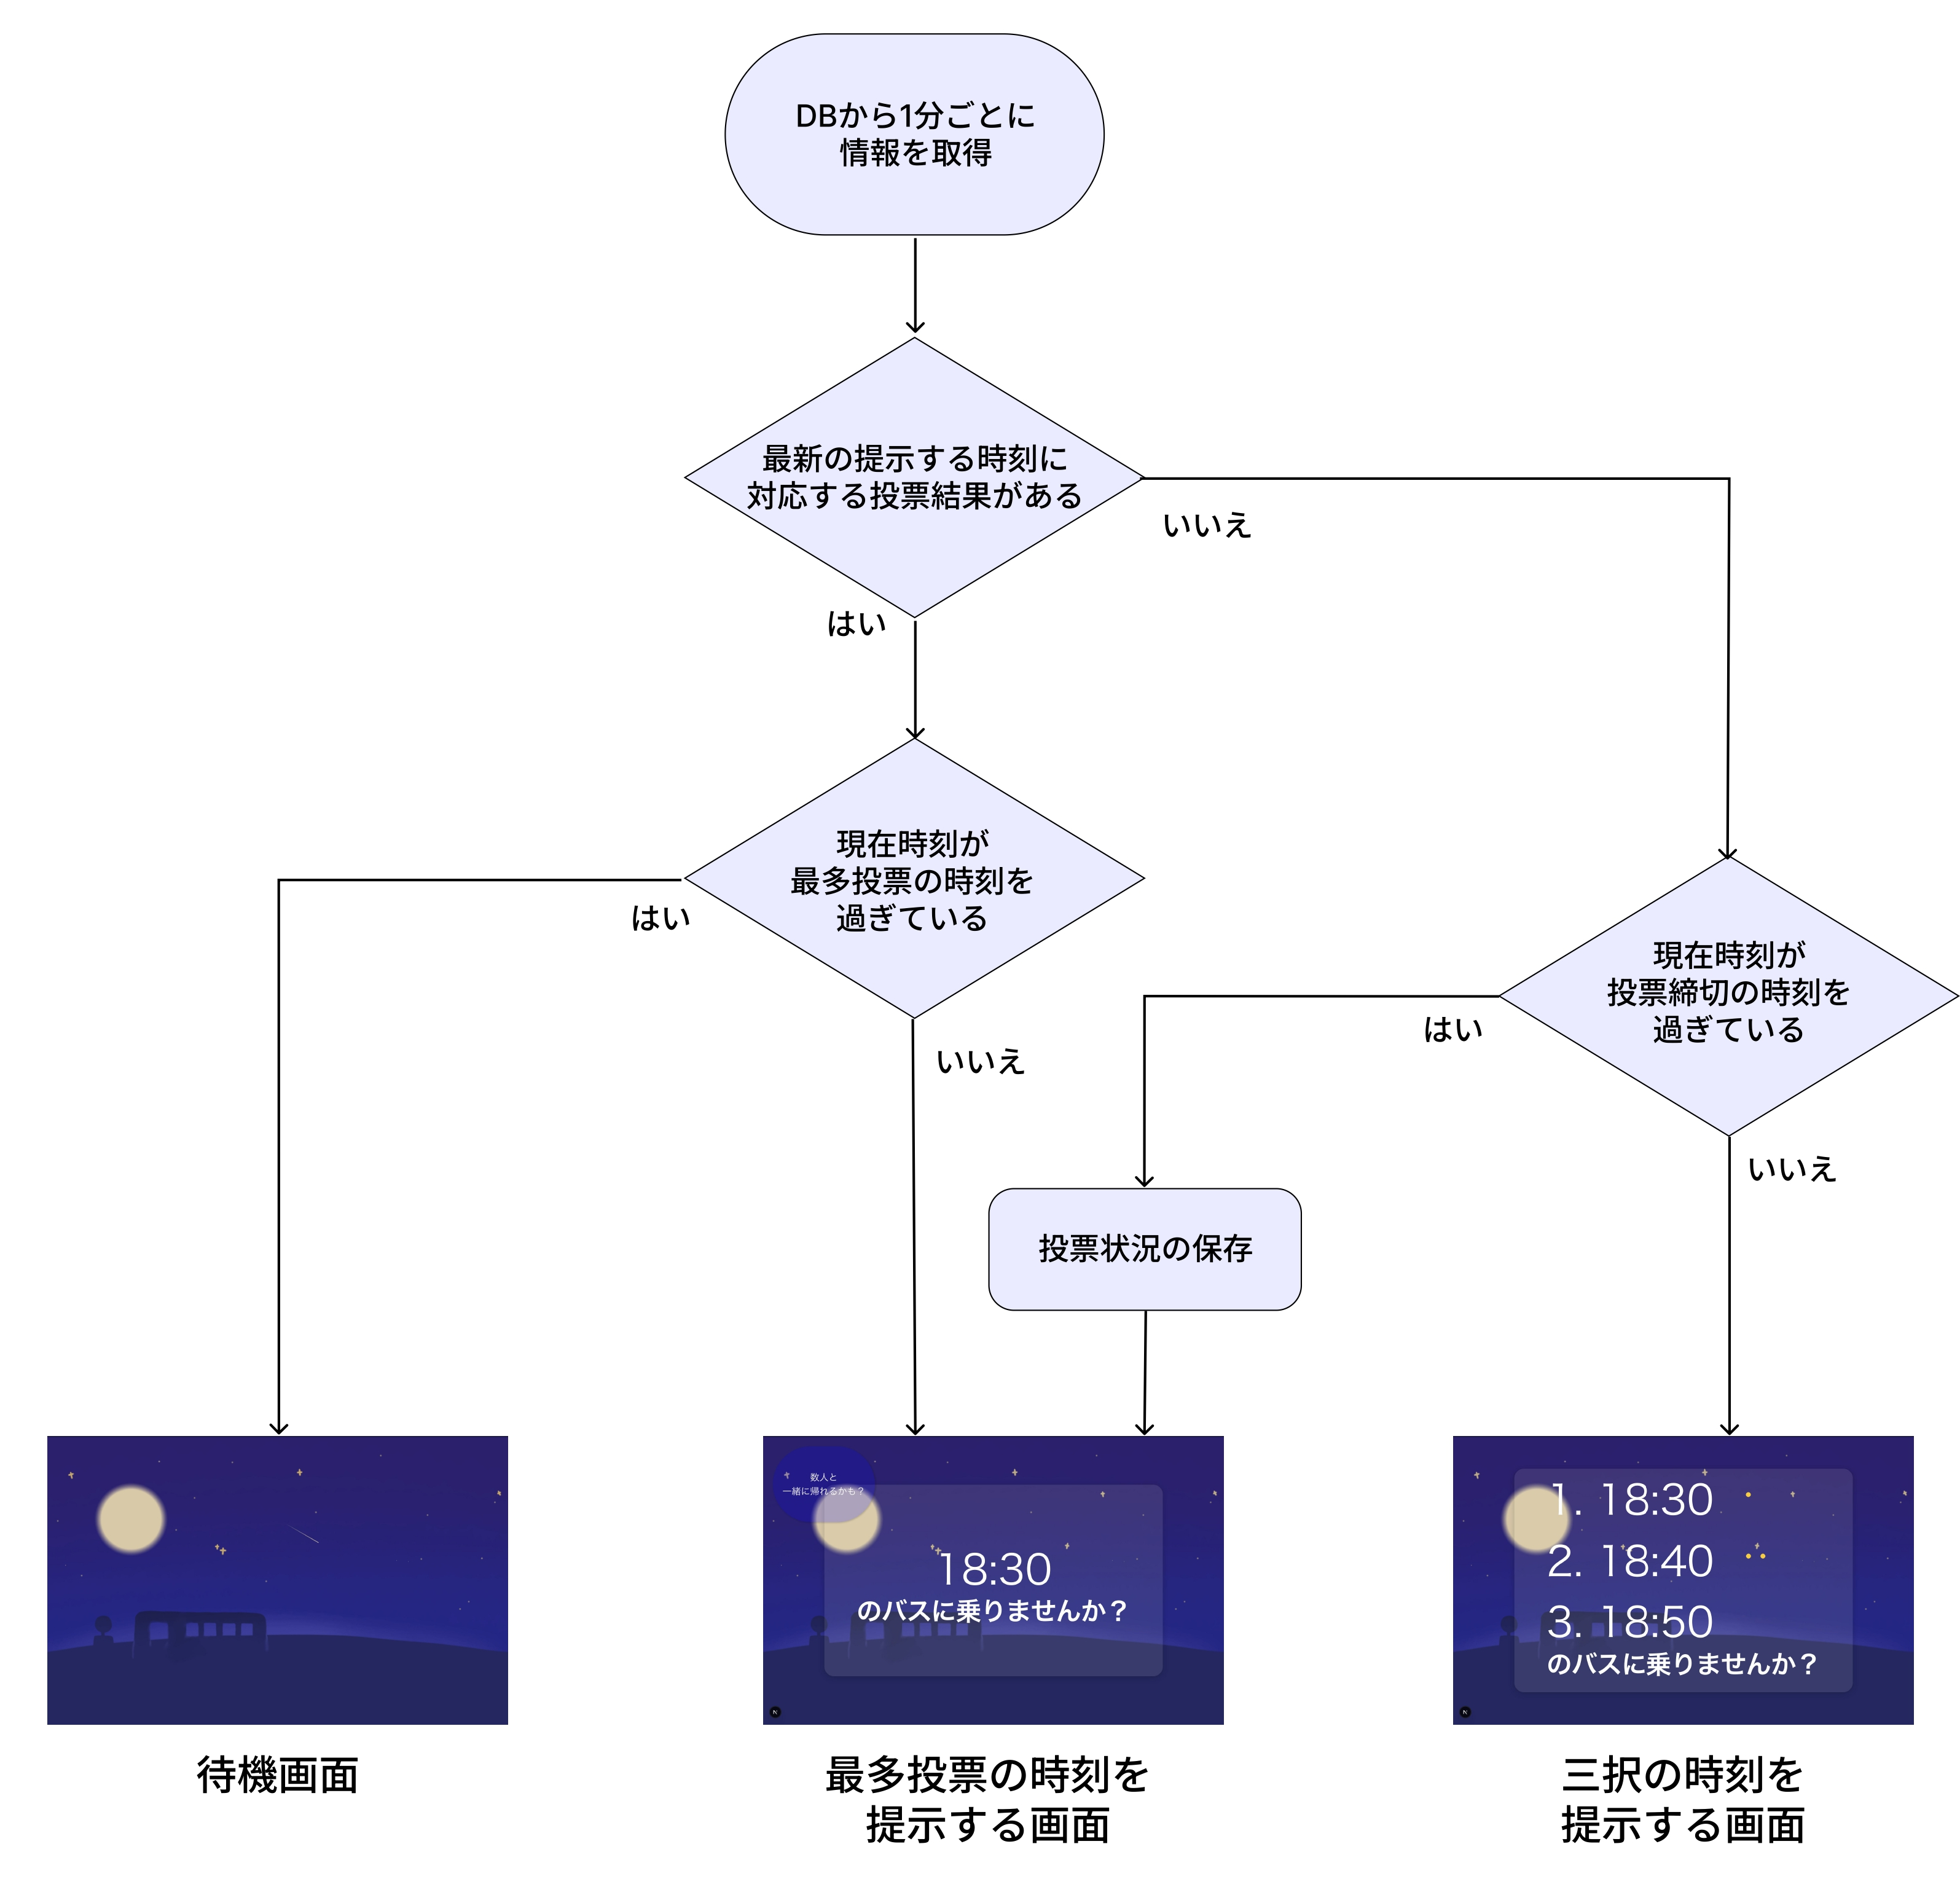
\includegraphics[width=0.9\linewidth]{fig/flow.jpg} % suzuki
  \caption{画面遷移}
  \label{fig:disflow}

\end{figure}

\subsection{三択の時刻を提示する画面}
この画面では三択の時刻と，それぞれの時刻への投票数を表示する．
実際の画面を図\ref{fig:selectDisplay}に示す．
この画面への遷移時には音声による通知を行い，画面表示の変化に気づきやすくしている．
また，投票状況を時刻横に丸の数として反映し，他の人の投票を参考に帰宅時刻の検討や変更ができる設計としている．
現在時刻が投票締切時刻をすぎた際に最多投票の時刻を提示する画面へと自動的に遷移する．

\begin{figure}[htb]
  \centering
  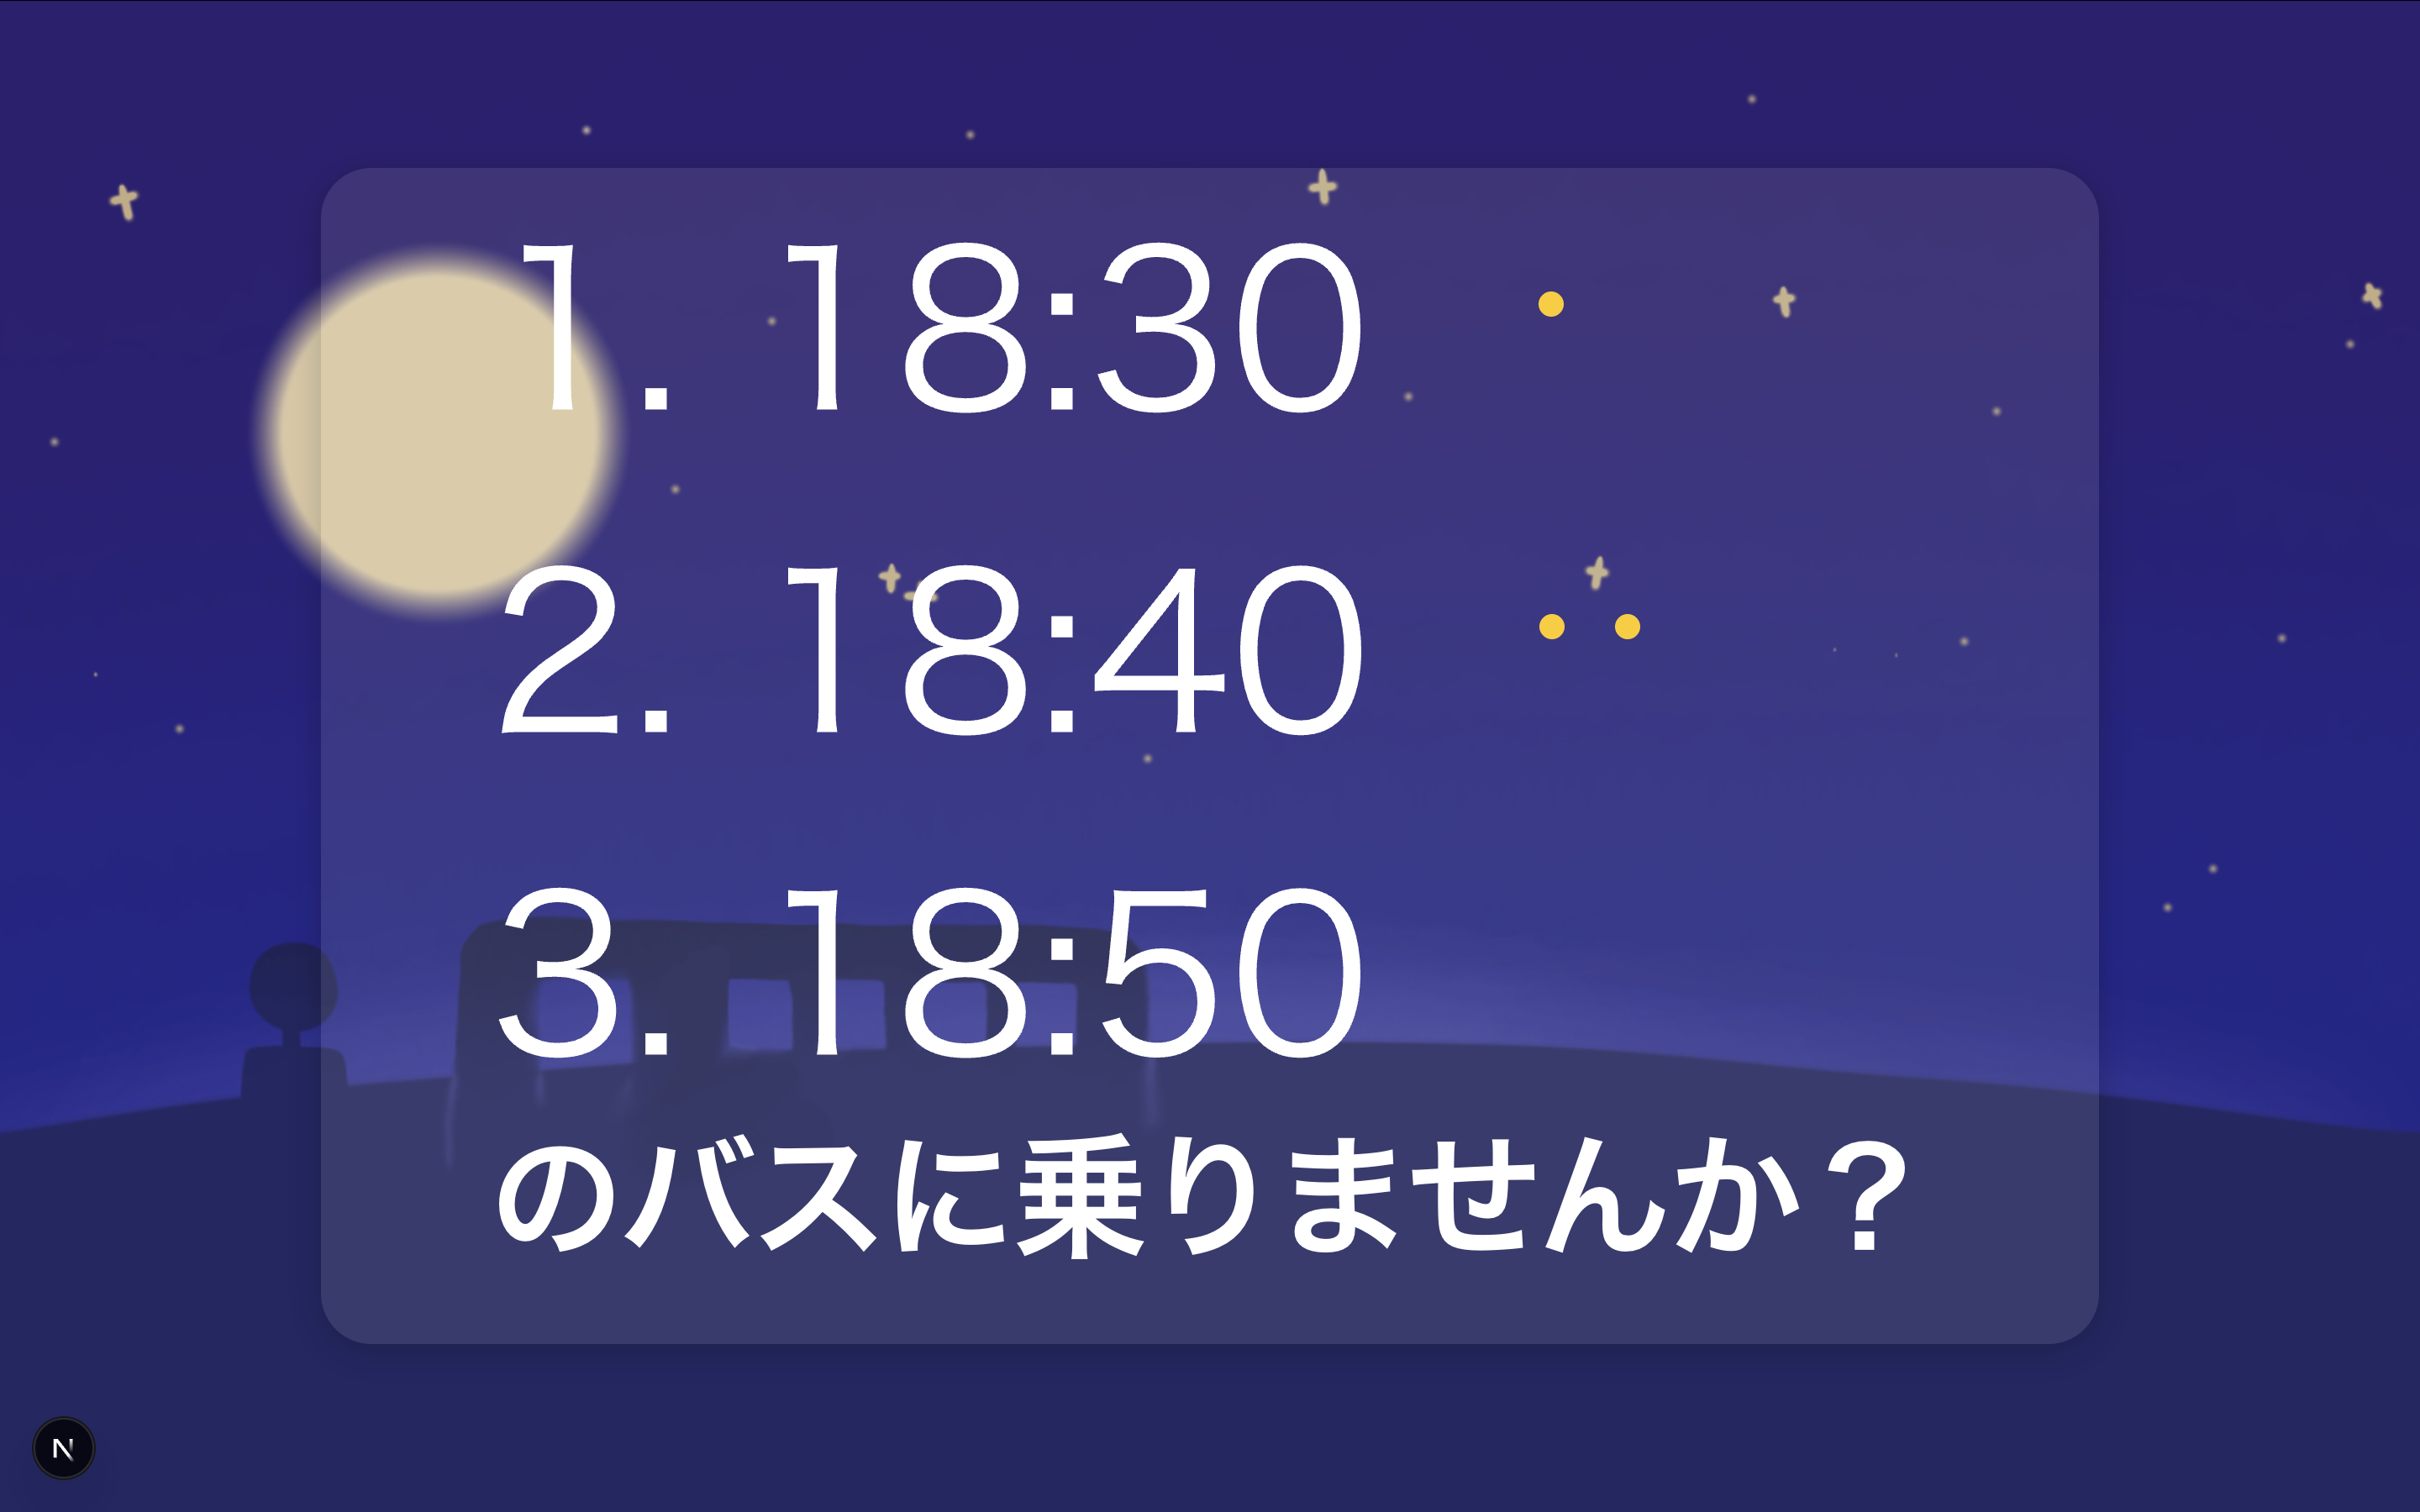
\includegraphics[width=0.7\linewidth]{selectDisplay.png} % suzuki
  \caption{三択の時刻を提示する画面}
  \label{fig:selectDisplay}

\end{figure}

本画面の設計にあたっては，設置環境や利用状況を踏まえた視認性および理解のしやすさに配慮した．
本画面は，共有スペースに設置された小型のモニターでの利用も想定し，離れた位置からでも内容を把握できるよう，時刻情報を画面内で大きく表示する設計とした．
また，各選択肢には数字を対応させ，ユーザが直感的に投票操作を行えるようにした．
加えて，「〜のバスに乗りませんか？」という表現を用いて，提示している時刻とバスの出発時刻の対応を一目で理解できるよう工夫した．
各時刻への投票状況は具体的な人数を数値で表示するのではなく，点の数として視覚的に表現した．
これにより，他者の選択傾向を直感的に把握できる一方で，人数の多寡を過度に強調せず，選択に対する心理的な圧力を和らげる意図がある．

また，本システムでは画面遷移への気づきを促すための一手段として音声通知を併用した．
通知に用いる音声には読み上げソフトである音読さん\cite{ondoku}を利用して作成した．
具体的には，「おすすめのバスの時刻が設定されました」という短い文言を読み上げた音声を用い，三択の提示画面へ遷移するタイミングで再生する．
音声内容は，ユーザに対して新たな情報提示が行われた事実のみを簡潔に伝える設計とし，周囲で行われている既存の対面コミュニケーションを過度に遮らないよう配慮した．
音声は画面遷移への気づきを促す目的で用い，具体的な時刻情報は表示画面に集約する設計とした．

この音声通知の作成にあたっては，画面遷移への気づきを促しつつも，通知時間が過度に長くならないよう配慮した．
具体的には，読み上げ音声の再生速度を標準よりやや速い設定とし，短時間で内容を伝えられるよう調整した．
また，周囲の環境音の中でも認識されやすいよう，比較的高めの声色を選択して音声を作成した．
以上のように，本システムにおける音声通知は，画面表示を中心とした情報提示を補完する手段として位置付けている．
\subsection{最多投票の時刻を提示する画面}

この画面では投票数が最も多かった時刻とその投票数を表示する．
実際の画面を図\ref{fig:resultDisplay}に示す．
この画面への遷移時に投票数の集計および表示を行う．
投票結果に基づき，最も帰宅行動につながりやすいと考えられる時刻を選択して表示する．
また，投票人数の表示方法を工夫し，声かけを行う際の心理的負担を軽減する設計とした．
現在時刻が表示している時刻をすぎた際に待機画面へと自動的に遷移する．
\begin{figure}[htb]
  \centering
  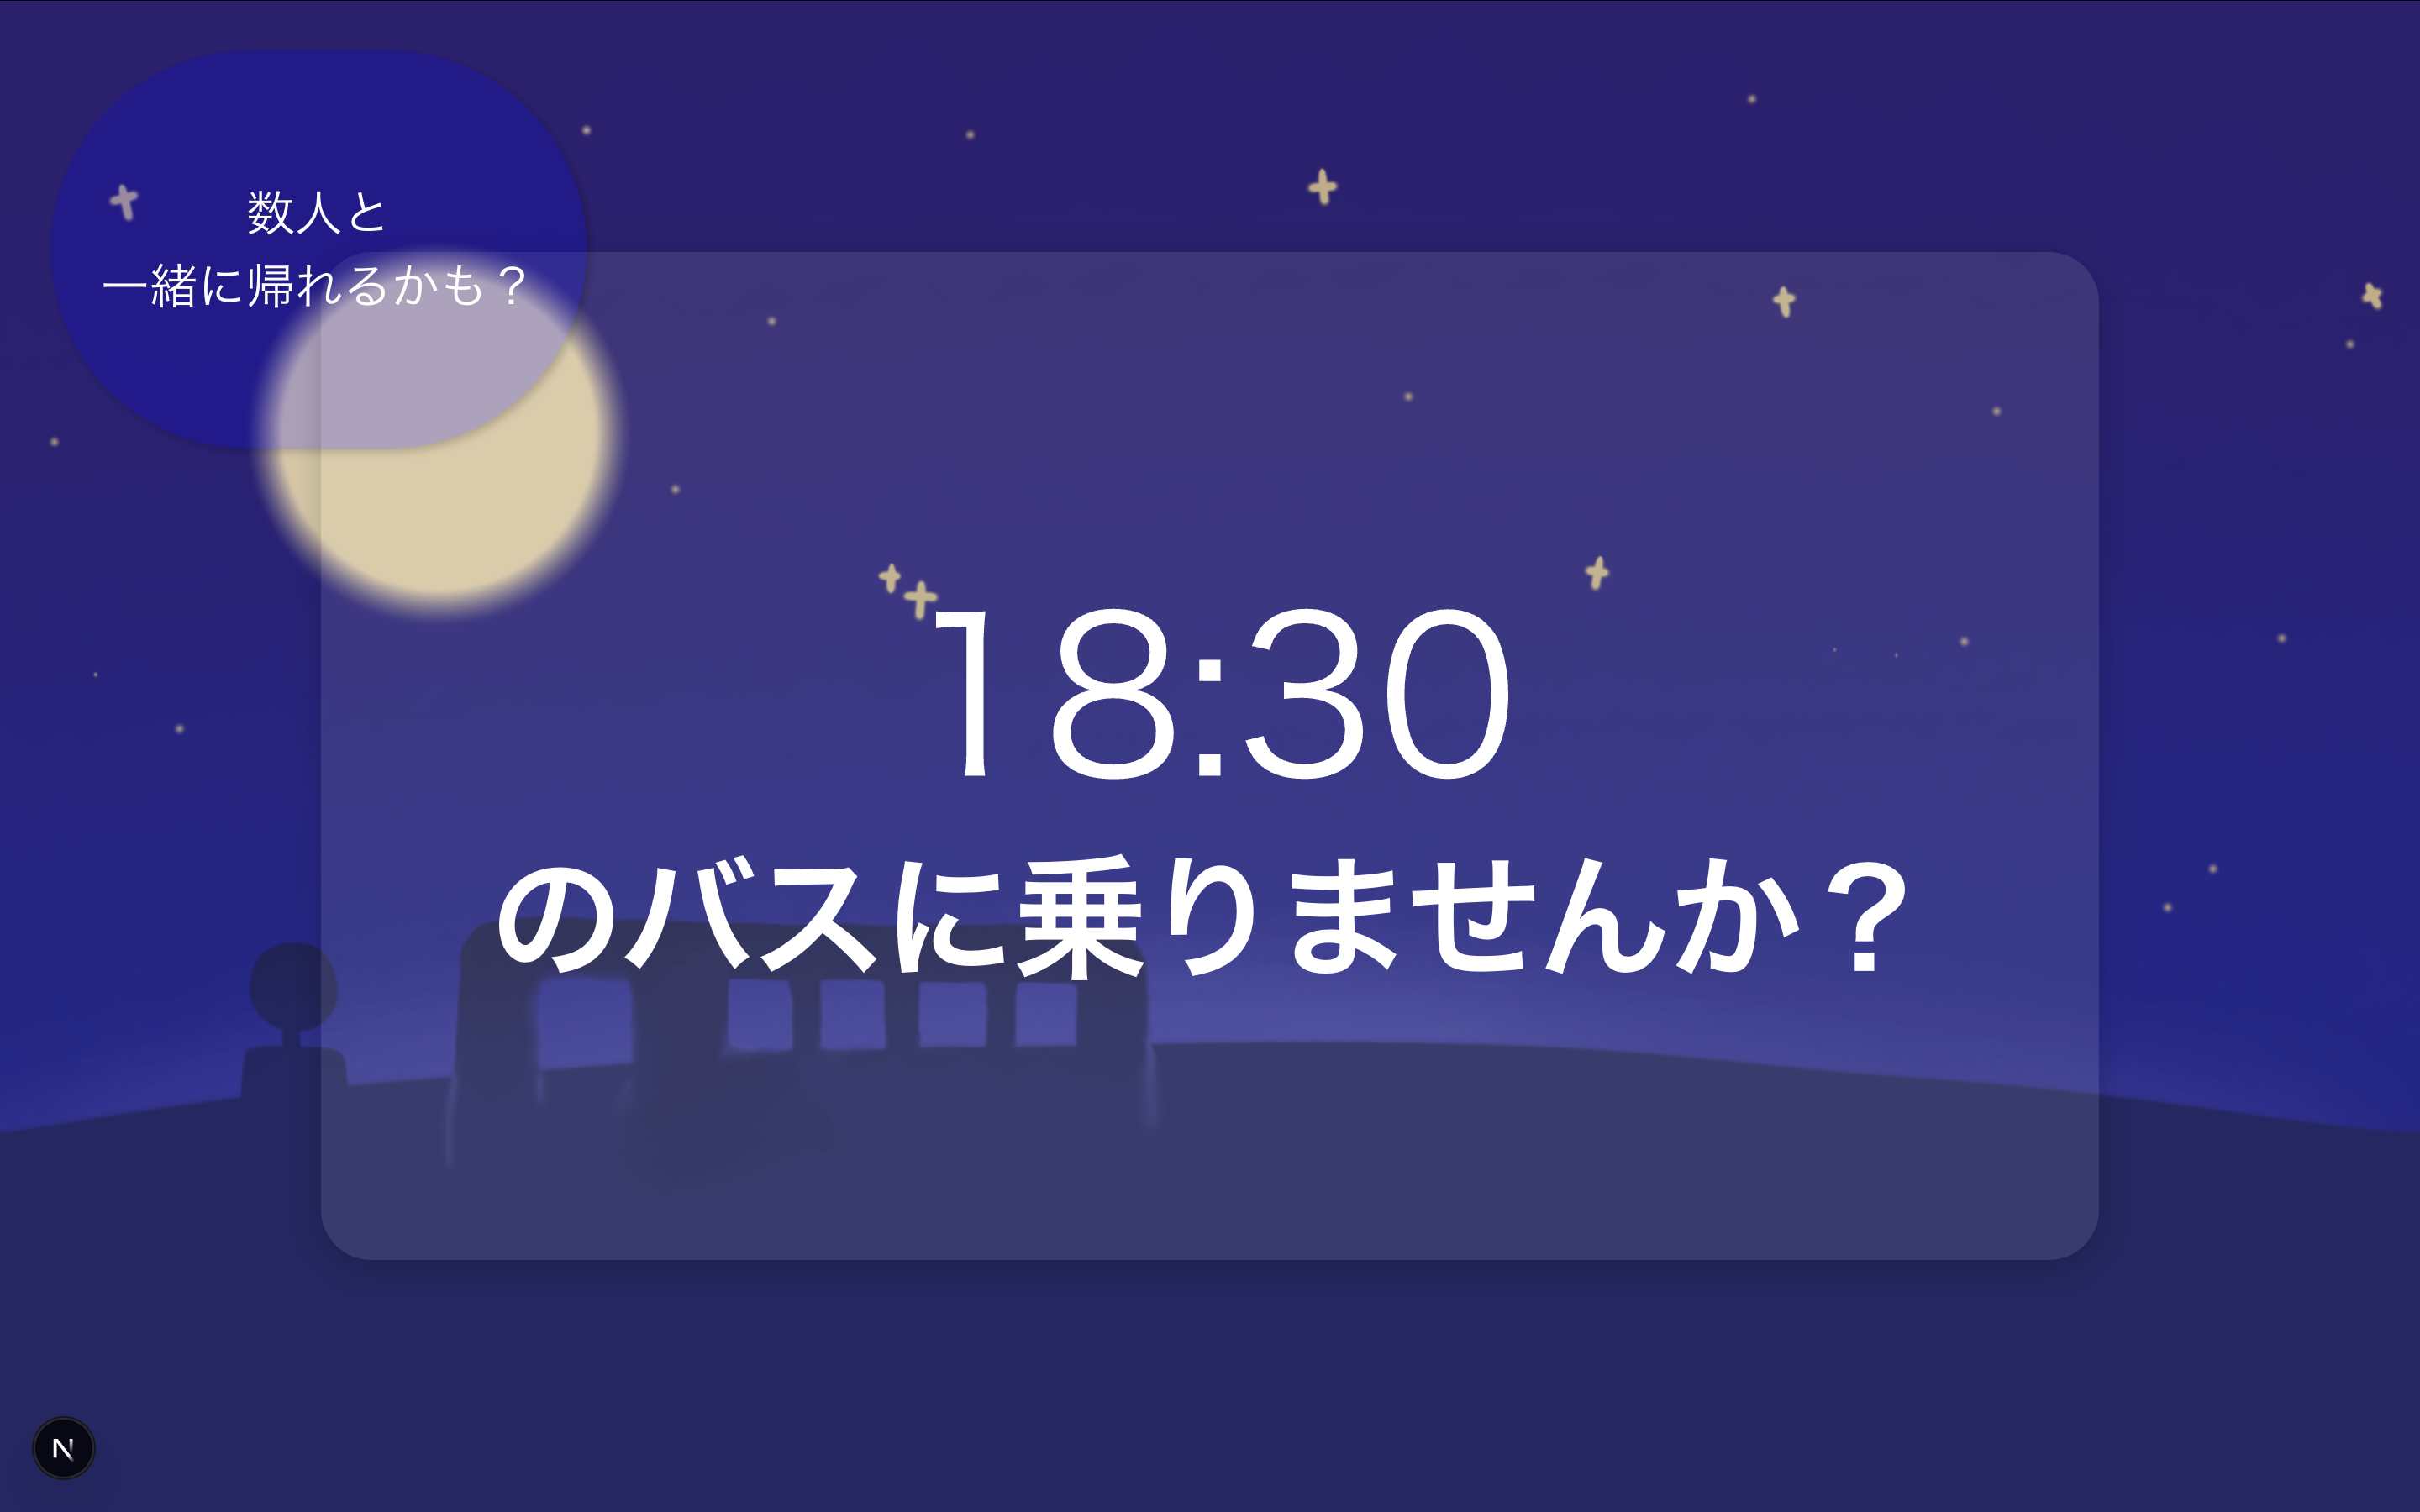
\includegraphics[width=0.7\linewidth]{resultDisplay.png} % suzuki
  \caption{最多投票の時刻を提示する画面}
  \label{fig:resultDisplay}

\end{figure}

% 本画面においても，離れた位置から内容を把握できるよう，帰宅時刻を画面内で大きく表示する設計とした．
% 本画面は，三択の投票結果をもとに，利用者の帰宅行動を一つの時刻へ収束させることを目的としている．
% 投票数が最も多かった時刻を強調して提示し，その時刻に帰宅可能な利用者が比較的多いと視覚的に示す設計とした．
% また，投票がなかった場合には，最も帰りやすいと考えられる帰宅推奨時刻に近い時刻を表示する．
% 同票の時刻が存在する場合には，各時刻の帰宅同行が成立する可能性が同程度であると判断し，より多くの利用者が帰宅行動を起こす前の時刻として，早い時刻を選択する．
% 一方で，投票人数に関する情報は，画面に近づいた際に確認できる程度の大きさとした．
% これにより，帰宅意思を持つ利用者が詳細情報を確認しやすくなる一方で，周囲にいる他の利用者に対して過度な情報提示とならないよう配慮している．
本画面においても，離れた位置から内容を把握できるよう，帰宅時刻を画面内で大きく表示する設計とした．
また，投票数が最も多かった時刻を強調して提示し，三択の投票結果の中で帰宅可能なユーザが比較的多い時刻を視覚的に示す．
一方で，投票人数に関する情報は，画面に近づいた際に確認できる程度の大きさとした．

本画面は，三択の投票結果をもとに，ユーザが帰宅しやすい時刻を一つに絞り込む目的で設計している．
したがって，投票がなかった場合には最も帰宅しやすいと考えられる帰宅推奨時刻に近い時刻を選択する．
同票の時刻が存在する場合には，各時刻の帰宅同行が成立する可能性が同程度であると判断し，より多くのユーザが帰宅行動を起こす前の時刻として，早い時刻を選択する．
また，投票人数の表示方法についても，声かけを行う際の心理的負担を抑える観点から設計している．

なお，本システムでは「おすすめの退室時刻」ではなく，利用者が目標とする行動の基準として「乗車すべきバスの時刻」を提示している．
これは，「この時刻までに出れば余裕をもって間に合う時刻」と「実際に出発すれば間に合う最終的な時刻」との間に存在する時間帯において，何も情報が提示されない状態を避けるためである．
また，この時間帯のみ表示内容や画面構成を切り替えると，利用者にとって表示規則が分かりにくくなる可能性がある．
そのため，本画面では一貫してバスの時刻を基準とした提示に専念し，実際に建物を出る時刻の判断は利用者に委ねる設計とした．


投票人数の表示方法については，人数の多寡によって表現を切り替えている(図\ref{fig:resultDisplays})．
具体的には，無投票の場合は人数表示を行わず，1票の場合には「数人と一緒に帰れるかも？」という抽象的な表現を用いた．
2票以上の場合には「〜人と一緒に帰れるかも？」と具体的な人数を示す．
これは，投票したユーザがその時刻に帰宅可能であると仮定し，「一緒に帰れる可能性」を提示し，声かけを行う際の心理的なハードルを下げる意図で設計した．

\begin{figure}[htb]
  \centering
  \subcaptionbox{無投票の場合}{
    
\includegraphics[width=0.3\linewidth]{0.png}}	% suzuki
  \hspace{3mm}
  \subcaptionbox{投票数が1の場合}{
    
\includegraphics[width=0.3\linewidth]{1.png}}	% suzuki 
  \hspace{3mm}
  \subcaptionbox{投票数が複数の場合}{
    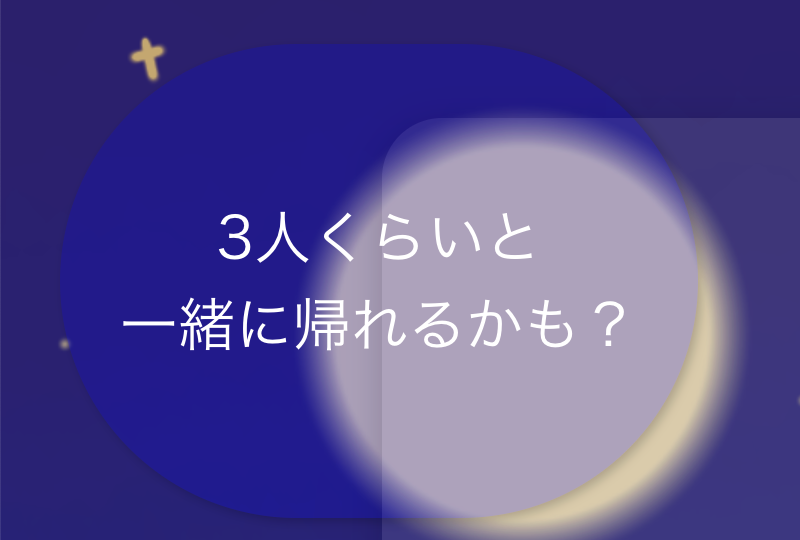
\includegraphics[width=0.3\linewidth]{3.png}}
  \caption{投票人数の提示箇所}
  \label{fig:resultDisplays}
\end{figure}
\subsection{待機画面}

% 以上の2つの画面でない状況を示す．
本画面は，三択の時刻を提示する画面および最多投票の時刻を提示する画面のいずれにも該当しない状態を明確に示すための画面である．
投票対象外の時間帯や，投票が開始される条件を満たしていない場合，および表示された投票結果の時刻を過ぎた場合に図\ref{fig:waitingDisplay}(\subref{fig:wait})のように表示される．
新たに三択の時刻が設定された際に三択の時刻を提示する画面へと自動的に遷移する．

また，システムが稼働中であると示すため，画面内に小さな動きを付与している．
これは，画面が停止していると誤認されるのを防ぎ，ユーザに対してシステムが正常に動作していると伝える意図がある．

さらに，投票対象外の時間帯であると視覚的に示すため，図\ref{fig:waitingDisplay}(\subref{fig:stop})のように画面全体を暗く表示している．
対象外の時間帯は，一般的に深夜および早朝とされる22:00から6:59までとし，この時間帯においては帰宅同行を促す情報提示を抑制する設計とした．

\begin{figure}[htb]
  \centering
  \subcaptionbox{条件外の場合の画面\label{fig:wait}}{
    
\includegraphics[width=0.4\linewidth]{fig/waitingDisplay.png}}	% suzuki
  \hspace{3mm}
  \subcaptionbox{対象外の時間の画面\label{fig:stop}}{
    
\includegraphics[width=0.4\linewidth]{fig/stoppingDisplay.png}}	% suzuki 
  \caption{待機画面}
  \label{fig:waitingDisplay}
\end{figure}

% \begin{figure}[htb]
%   \centering
%   \subcaptionbox{三択の時刻}{% % suzuki
%     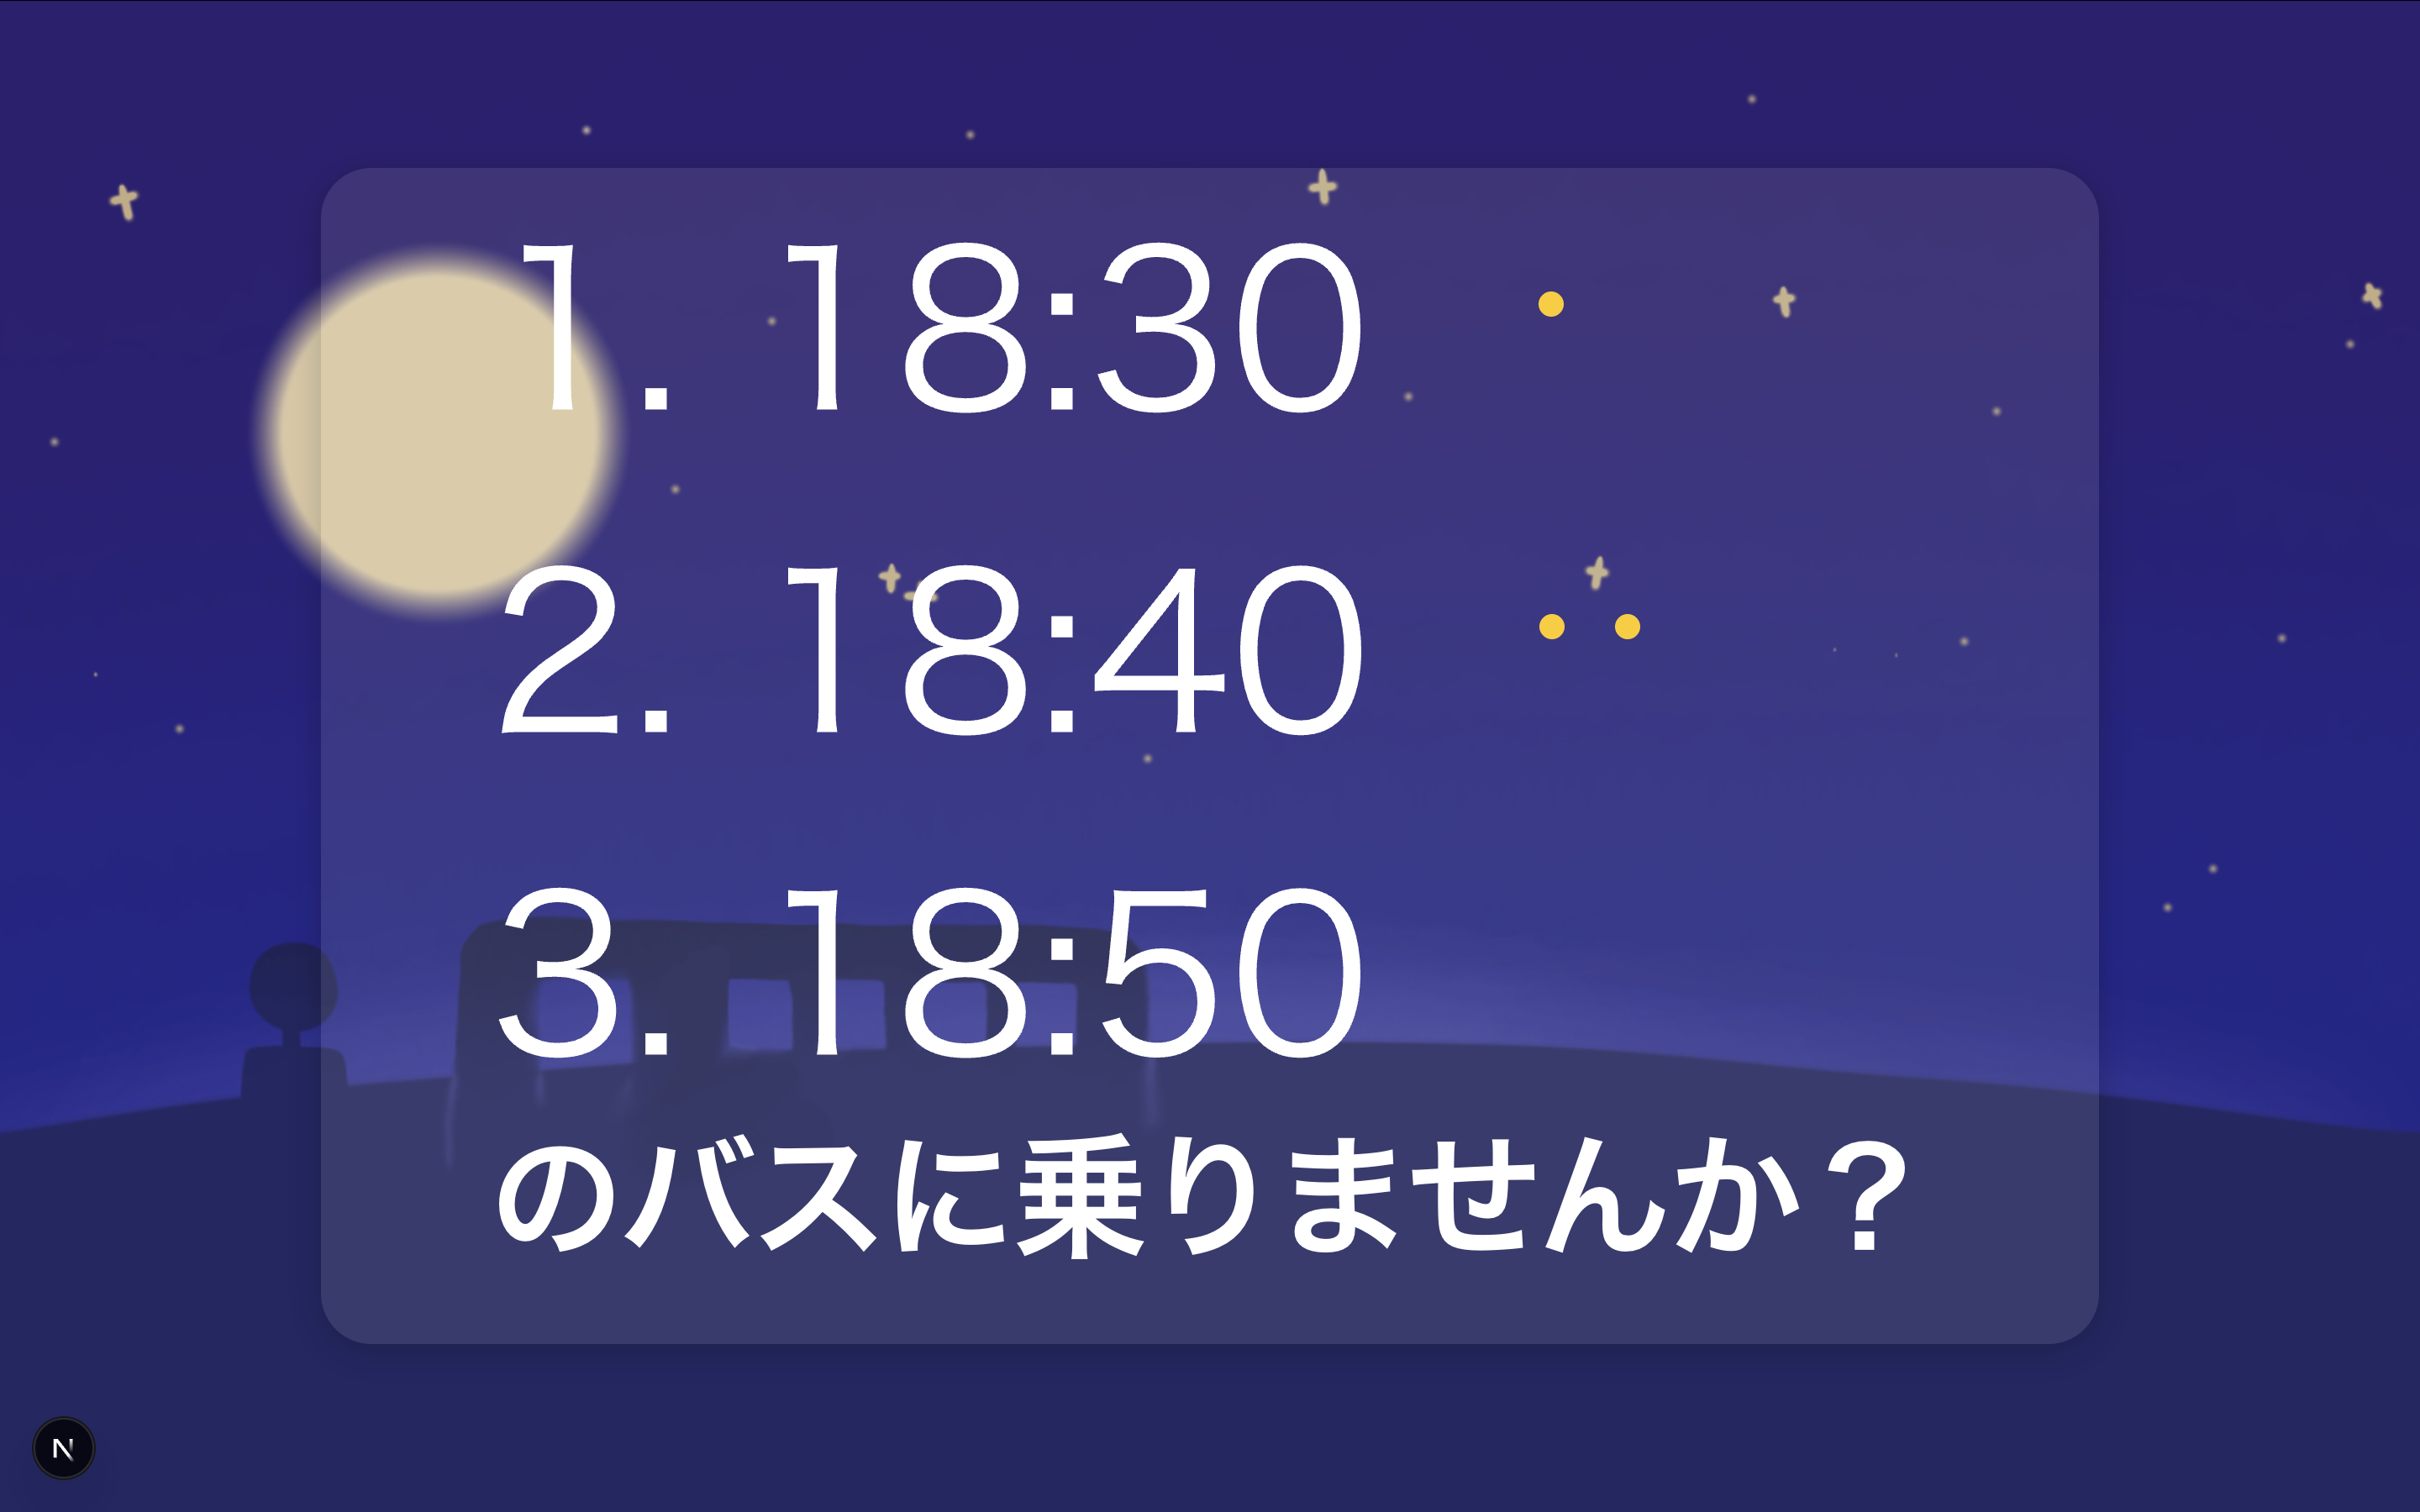
\includegraphics[width=0.4\linewidth]{selectDisplay.png}}	% suzuki
%   \hspace{3mm}
%   \subcaptionbox{最多投票の時刻}{%	% 良く考えたら投票人数による表示の違い全部載せた方がいいのでは？
%     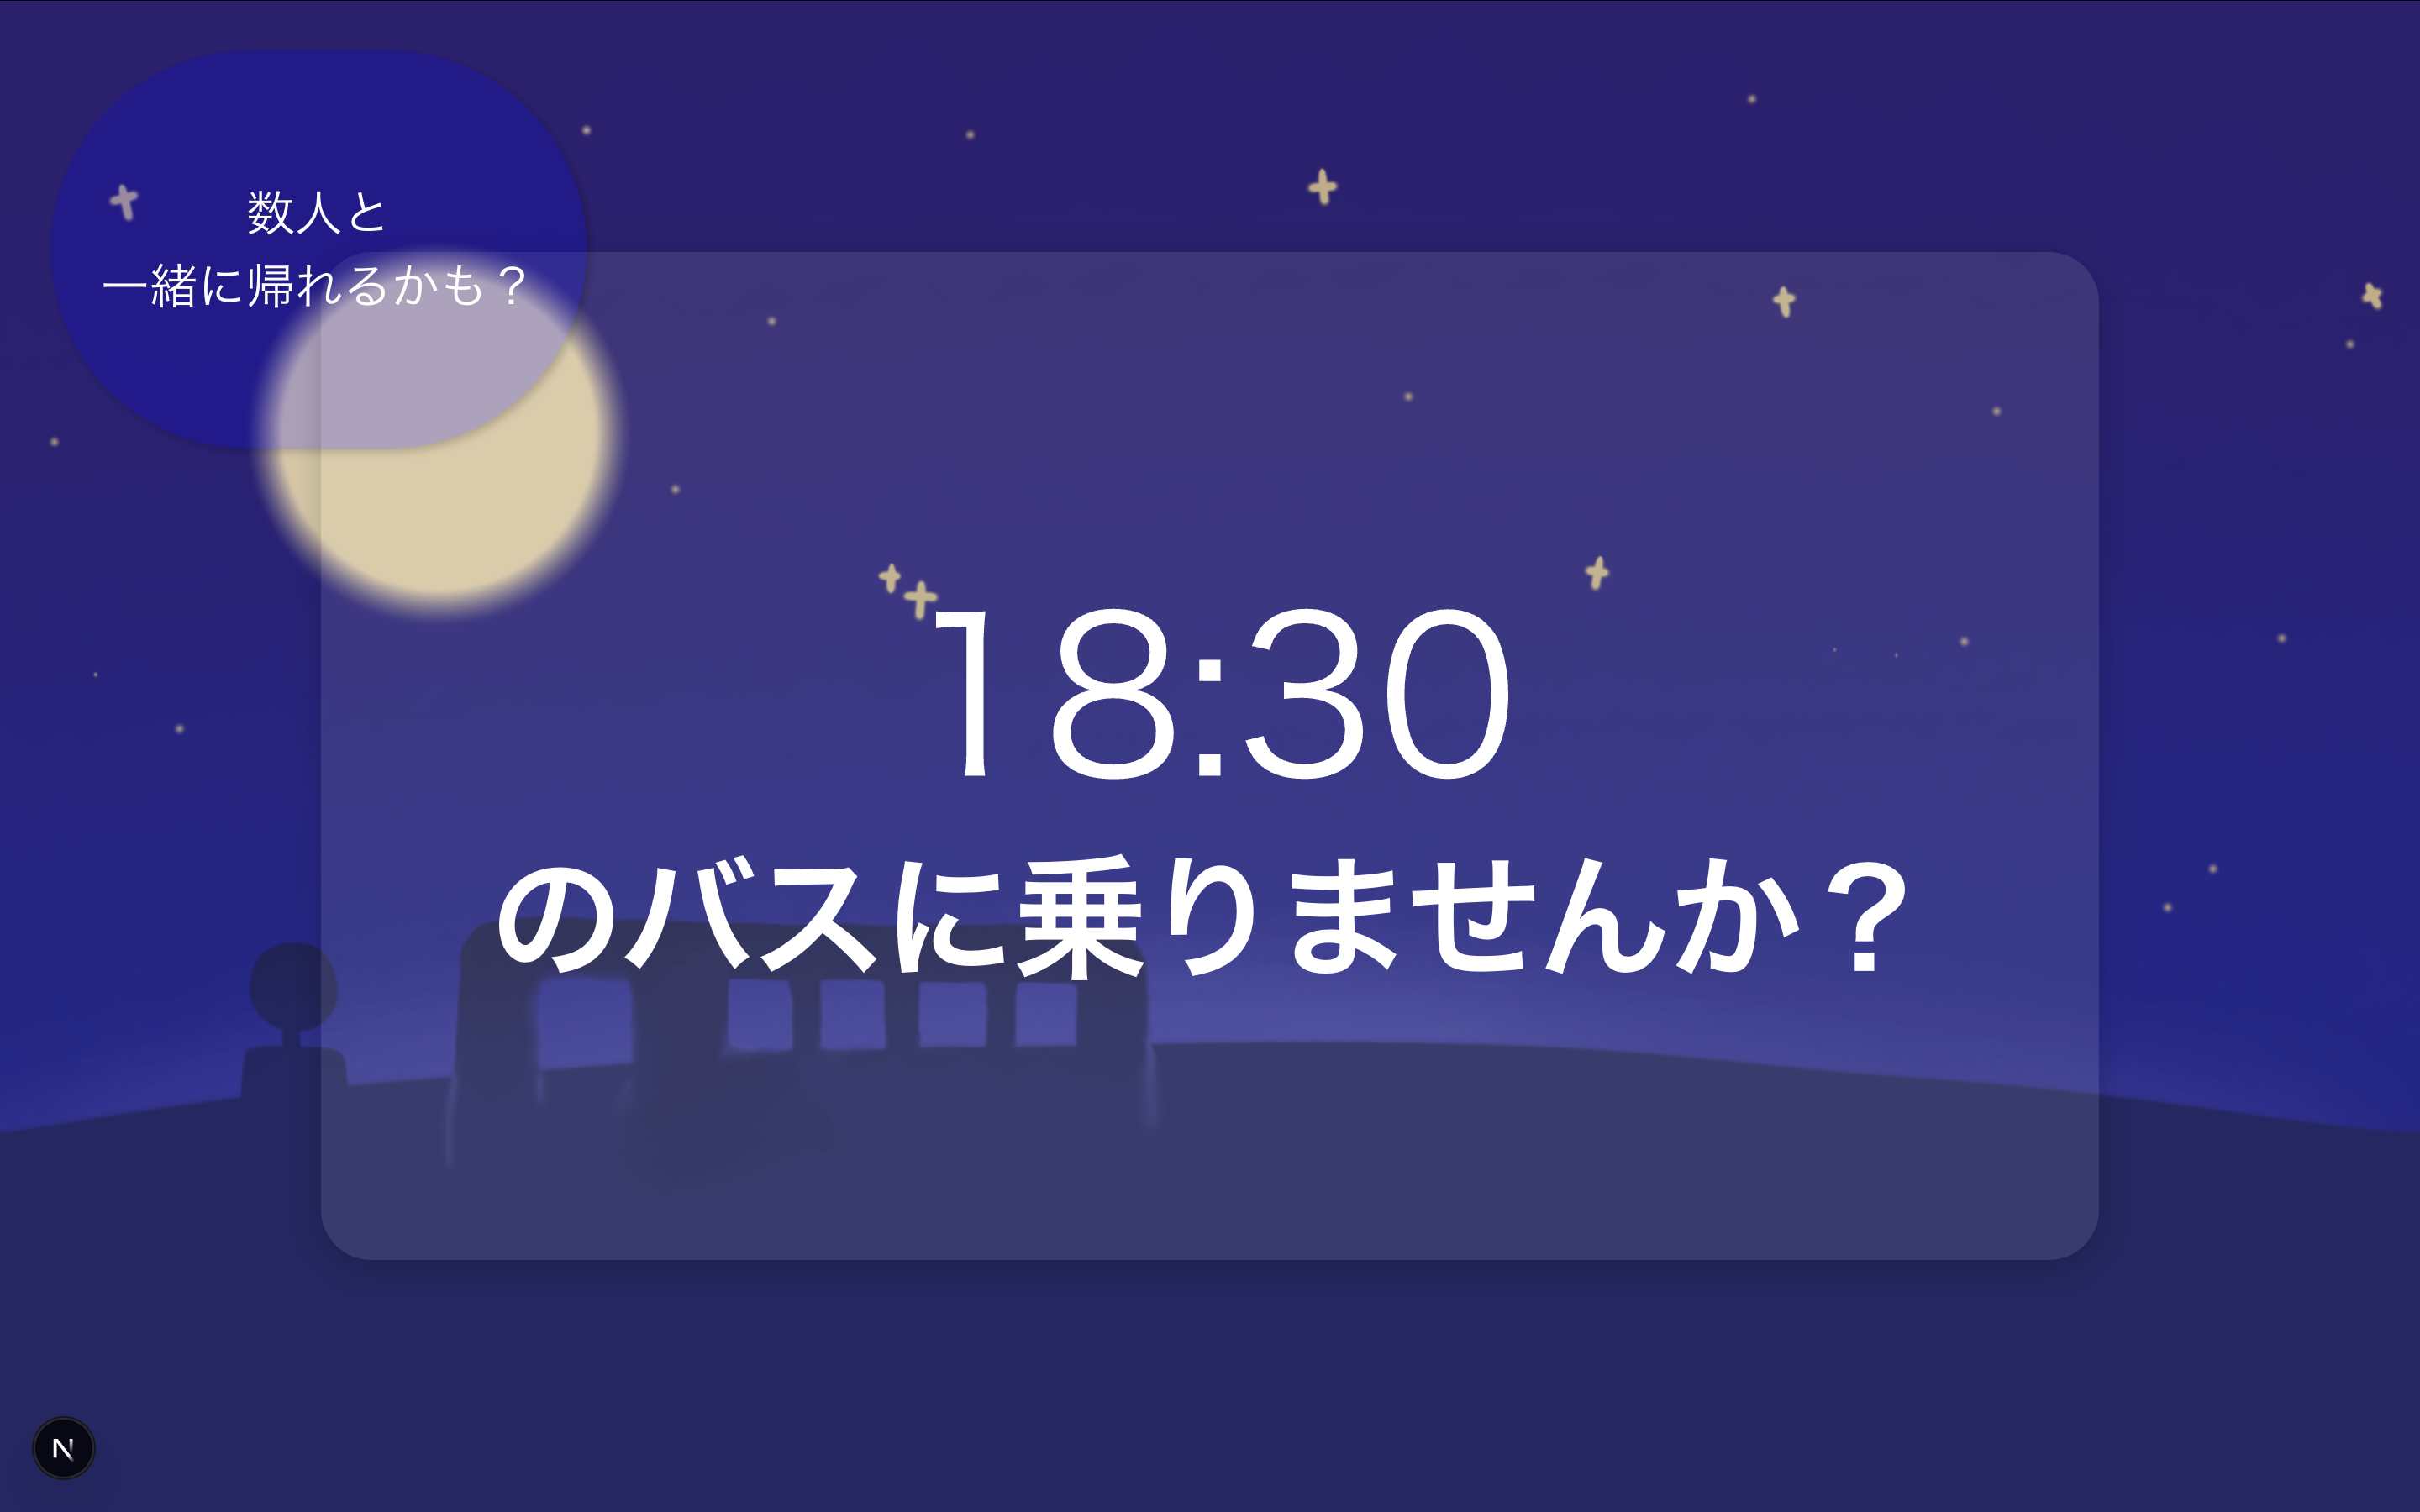
\includegraphics[width=0.4\linewidth]{resultDisplay.png}}	% suzuki 
%   \caption{時刻の提示を行う画面}
%   \label{fig:2}
% \end{figure}

% バックエンドの話も一部ここに持ってこよう
\section{組織内コミュニケーションツールでの投票}
本システムでは，研究室内で使用されているチャットツールであるSlackを採用し，SlackBotを用いてダイレクトメッセージ(以下DM)の送信および投票の受付を実現した．
%

% 帰宅推奨時刻の算出時に抽出した最多区間内のメンバに時刻情報を含んだダイレクトメッセージを送信し投票を促す．
% これによりユーザ側から近しい時刻に帰りそうな具体的なメンバを分からない状態にし，メンバ以外へのコミュニケーションの発生も狙った．

最多区間内に含まれるユーザは，帰宅推奨時刻付近で帰宅する可能性が高いと考えられる．
そのため，本システムでは，これらのユーザを帰宅同行の中心的な候補として位置付け，Slackを用いたDMの送信対象としている．
これにより，帰宅同行の可能性が低いユーザへの不要な通知を避けつつ，実際に同行が成立しやすいユーザに対して重点的にアプローチできる設計としている．

DMでは，「乗れそうなバスを選択してください」という文言とともに，算出されたバスの時刻を番号付きの選択肢として提示する．
\begin{figure}[htb]
  \centering
  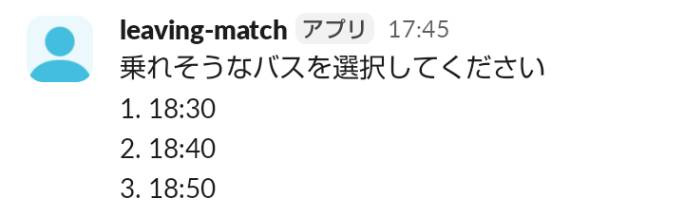
\includegraphics[width=0.6\linewidth]{slack.jpg} % suzuki
  \caption{SlackBotとのDMのスクリーンショット}
  \label{fig:slack}

\end{figure}

例えば三択の場合には，
\begin{description}
  \itemindent=1zw
  \itemsep=0mm
  \parsep=0mm
  \item 1. 19:30
  \item 2. 19:45
  \item 3. 20:00
\end{description}
のように表示され，二択の場合には
\begin{description}
  \itemindent=1zw
  \itemsep=0mm
  \parsep=0mm
  \item 1. 19:45
  \item 2. 20:00
\end{description}
のように提示される．
選択肢数に応じて表示を自動的に切り替え，ユーザは常に同じ操作感で投票を行える．
%同一ユーザの複数投票の扱い 投票変更可

また，投票は$1\sim$3の数字を入力させ打ち間違いを減らし，ユーザの手間を減らす設計にした．
複数の時刻への投票を可能とし，帰宅時刻を柔軟に変更できるユーザがより投票しやすい設計にした．
同一ユーザによる複数回の投票が行われた場合には，最新の投票内容のみを有効とする．


DMの送信および投票受付は，三択の時刻が算出された時点で開始され，最多投票の時刻が決定するまでの間に行われた投票のみを集計対象とする．
この時間帯以外に送信されたメッセージは集計されない．
なお，投票の受付から集計までの一連の処理は，すべてユーザとSlackBotとの個別DM内で完結する設計としている．
これによりユーザ側から近しい時刻に帰りそうな具体的なメンバを分からない状態にし，メンバ以外へのコミュニケーションの発生も狙った．



% \section{グラマーモデルへの適用}

% \subsection{グラマーモデルへの適用方法の提案}

% \subsection{データ構造}

% \subsection{検索アルゴリズム}

% \subsection{登録アルゴリズム}

% \subsection{削除アルゴリズム}

% Local Variables: 
% mode: japanese-LaTeX
% TeX-master: "root"
% End: 
